\documentclass{article}
\usepackage{amsmath}
\usepackage[pdflax]{graphicx}
\begin{document}
\begin{center}
    {\bf Restricted Boltzmann Machine}
\end{center}
Implemented restricted Boltzmann Machine, and experimented with subset of the MNIST.
Only considered 2,3,4 as train set from MNIST for the purpose of the time. I used
400 hidden unit, 0.05 learning rate, and 0.8 final momentum.
Here is some sample of data that it generated after running 25 epoch.
{\bf Generating data}\\
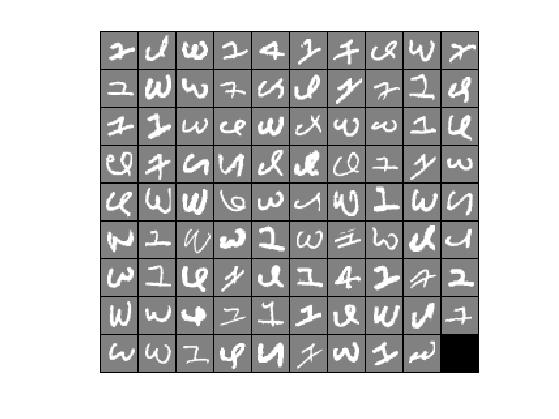
\includegraphics[scale=0.4]{rbm_h400_l0.005_m0.8/subdata.jpg}
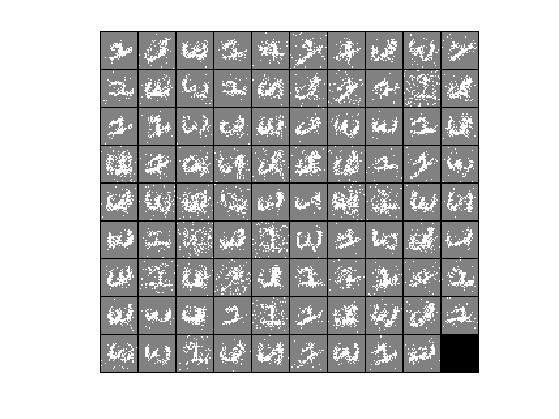
\includegraphics[scale=0.4]{rbm_h400_l0.005_m0.8/gensubdata_rbm.jpg}\\
First image is the actual subdata, and second iamge is the subdata that
rbm tried to generate.\\
{\bf Classification}\\
After running rbm to train as shown above, and used the weight from rbm as
initial weights to learn the neural network.\\
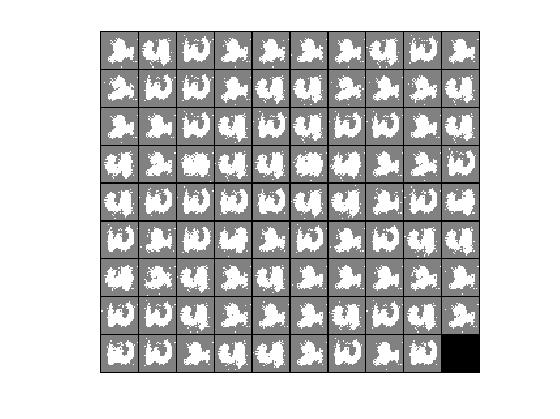
\includegraphics[scale=0.4]{rbm_h400_l0.005_m0.8/gen_classify.jpg}\\
This image is the image that it generated using the weights after it learned to
classify. This network got 0.045 error for train set, and 0.041 error for the test
set.\\\\
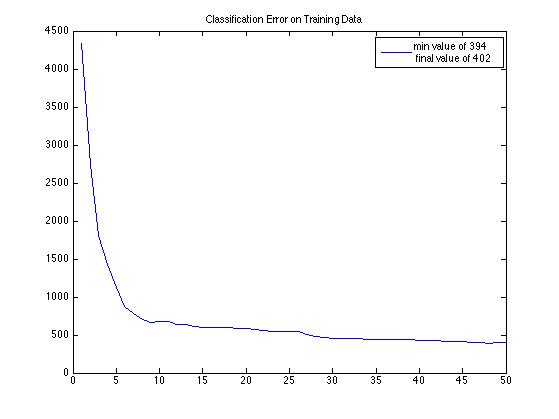
\includegraphics[scale=0.4]{rbm_h400_l0.005_m0.8/classErrTrain.jpg}
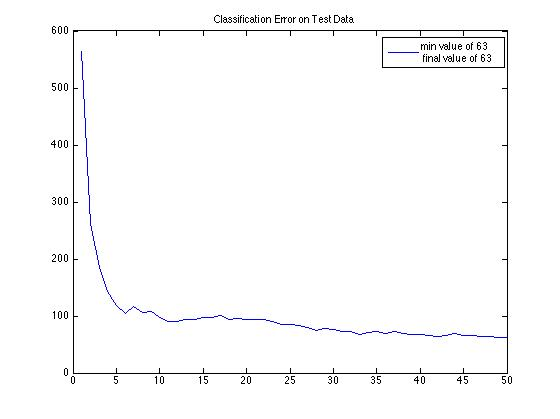
\includegraphics[scale=0.4]{rbm_h400_l0.005_m0.8/classErrTest.jpg}\\
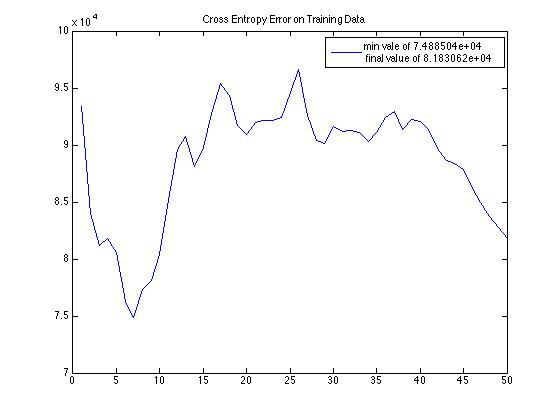
\includegraphics[scale=0.4]{rbm_h400_l0.005_m0.8/crossEntroTrain.jpg}
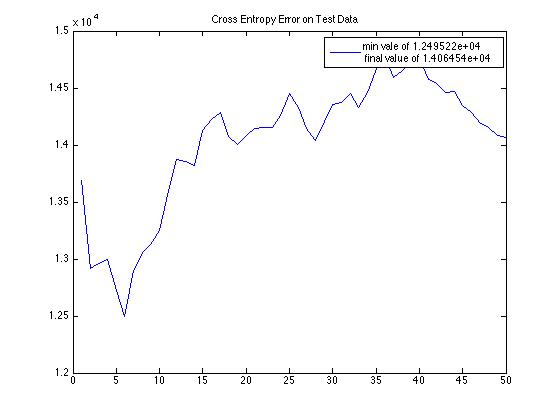
\includegraphics[scale=0.4]{rbm_h400_l0.005_m0.8/crossEntroTest.jpg}\\





\end{document}


